

%WMWMWMWMWMWMWMWMWMWMWMWMWMWMWMWMWMWMWMWM
% BACKGROUND
%WMWMWMWMWMWMWMWMWMWMWMWMWMWMWMWMWMWMWMWM
% figure: reform 
\begin{figure}[H]\centering
	
	%\input{../../analysis/graphs/paper/tikz_reform_extended_pre_and_post_birth.tex}
	%\includegraphics[width=\linewidth]{../../analysis/graphs/paper/tikz_reform_extended_pre_and_post_birth.tikz}
	%\includegraphics[width=0.9\linewidth]{../../analysis/graphs/paper/tikz_reform_short_post_birth.tikz}
	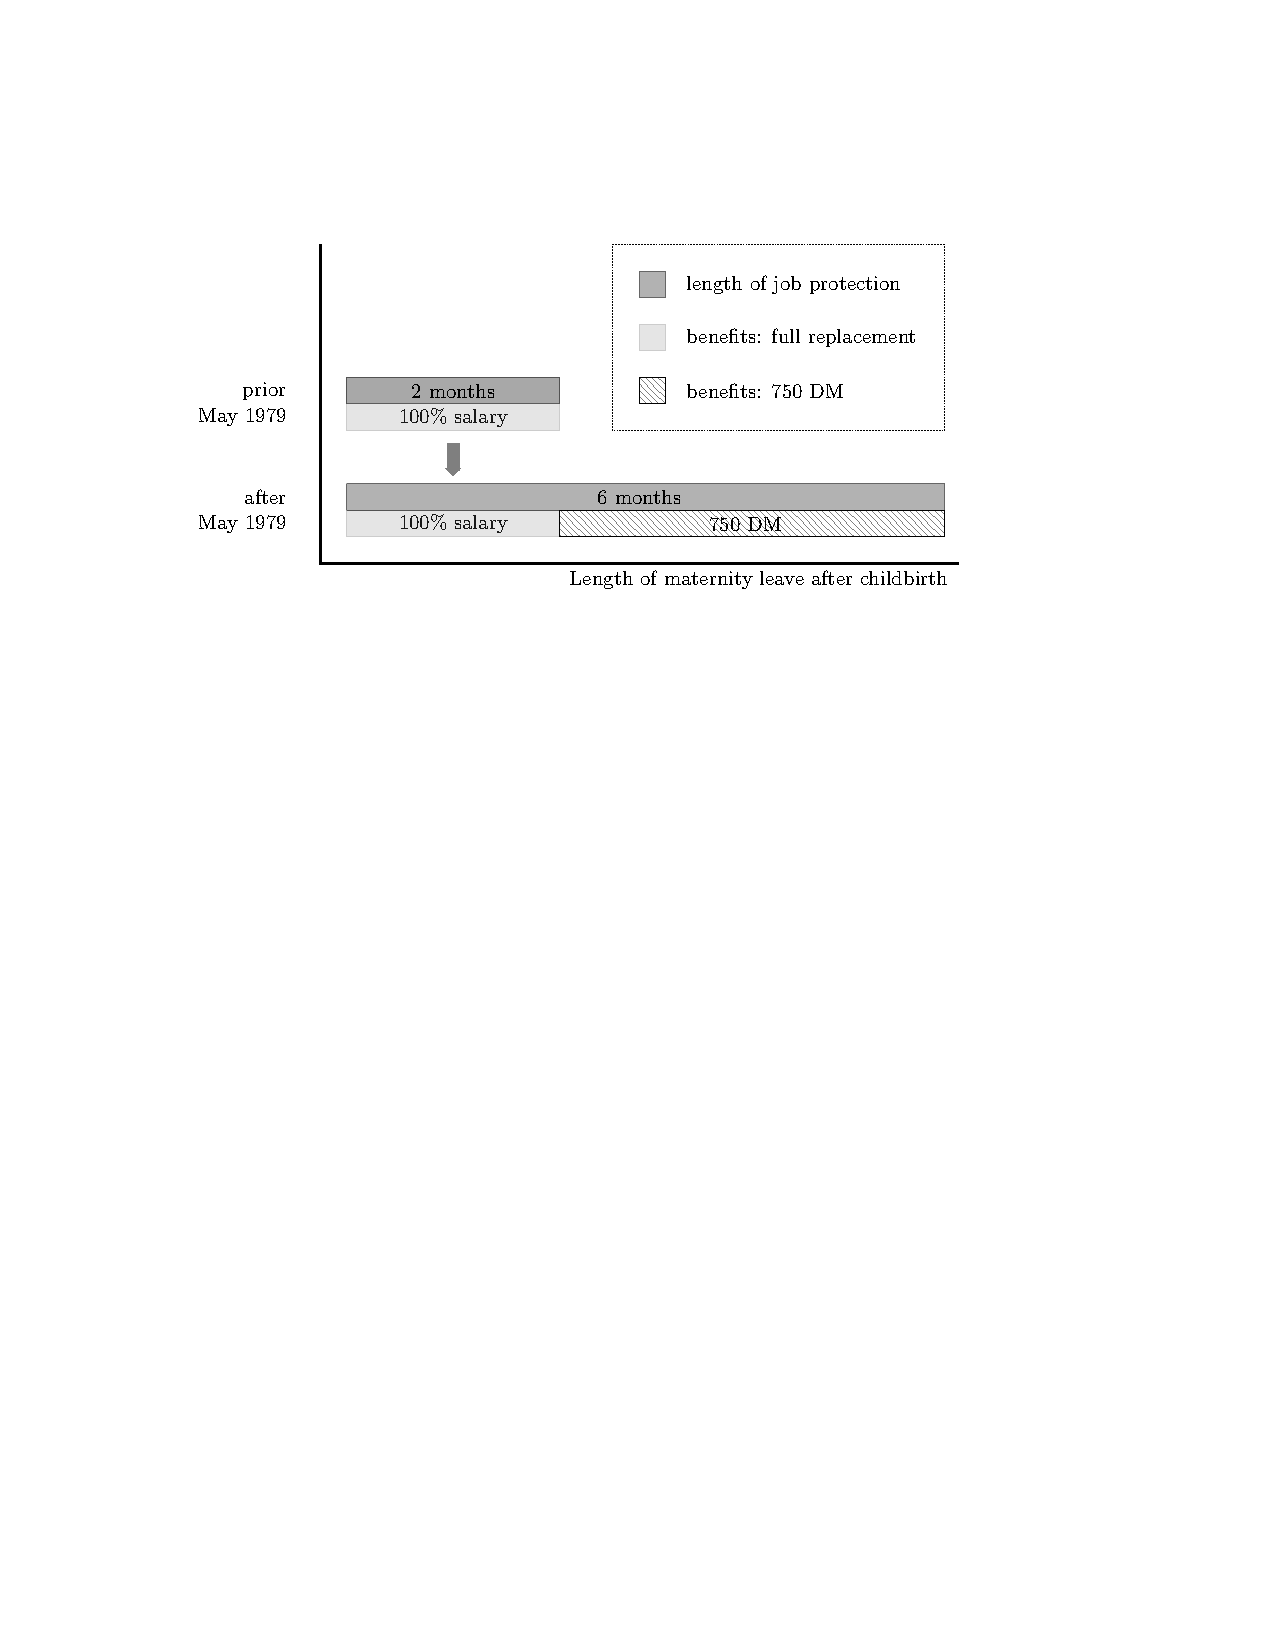
\includegraphics[width=0.9\linewidth]{SOEP/Reform_shortened.pdf}
	\begin{minipage}{0.9\linewidth}
		\caption{1979 reform in ML legislation in the Federal Republic of Germany}\label{fig_mlch: MLreform}
		\scriptsize{\emph{Notes:} The figure describes the legislative change in the length of job protection and ML, which took place in the Federal Republic of Germany in 1979. The reform increased post-birth ML from eight weeks to six months, while keeping the initial structure of the period from six weeks before until eight weeks after childbirth unchanged (mother protection period).\newline \textit{Source: }The figure is based on information from \cite{Dustmann2012}, \cite{DIW2002}, \cite{schonberg2014expansions} as well as \cite{zmarzlik1999mutterschutzgesetz}.}
	\end{minipage}
\end{figure}
%--------------------------------------------
% % figure: Bundesgesetzblatt und Familienministerin
% \vspace*{\fill}
% \begin{figure}[H]\centering
% 	\caption{Introduction of the maternity leave law}\label{fig_mlch: bundesgesetzblatt_antjehuber}
% 	\begin{subfigure}[h]{0.48\linewidth}\centering%\caption{Federal law gazette}
% 		\includegraphics[width=\linewidth]{paper/bundesgesetzblatt_coverpage.png}
% 	\end{subfigure}
% 	\begin{subfigure}[h]{0.48\linewidth}\centering%\caption{Federal Minister of Family Affairs Antje Huber} 
% 		\includegraphics[width=\linewidth]{paper/antje_huber.jpg}
% 	\end{subfigure}
% 	\begin{minipage}{\linewidth}
% 		\scriptsize{\emph{Notes:} On the left, the figure shows the ML law as published in the Federal law gazette. On the right, one can see the Federal Minister of Family affairs Antje Huber at the introduction of the ML law, which was published by the Ministry on the occasion of 30 years of the Federal Ministry of Women.\newline \emph{Source:} Bundesanzeiger Verlag and Federal Ministry of Justice and Consumer Protection (\hyperlink{http://www.bgbl.de/xaver/bgbl/start.xav?startbk=Bundesanzeiger_BGBl&jumpTo=bgbl179s0797.pdf}{BMJV}) and Federal Ministry for Family Affairs, Senior Citizens, Women and Youth (\hyperlink{https://twitter.com/bmfsfj/status/745513281989677058}{BMFSFJ}).}
% 	\end{minipage}
% \end{figure}
% \vspace*{\fill}\clearpage




%WMWMWMWMWMWMWMWMWMWMWMWMWMWMWMWMWMWMWMWM
% DATA
%WMWMWMWMWMWMWMWMWMWMWMWMWMWMWMWMWMWMWMWM
%figure TOP 5 Diagnoses across age groups
\vspace*{\fill}
\begin{figure}[H]\centering
	\includegraphics[width=0.9\linewidth]{paper/top5diagnoses_across_agegroups.pdf}
	\begin{minipage}{0.9\linewidth}
		\caption{Five main diagnoses of inpatients aged 0 to 35 in 2014}\label{fig_mlch: top5diagnosis_in_2014_across_agegroups}
		\scriptsize{\emph{Notes:} The figure shows the incidence distribution across different age brackets of the top five diagnoses for inpatients aged 0 to 35 in 2014. Diagnoses associated with pregnancy, childbirth, and the puerperium are not taken into account in this representation. The large remainder in the age bracket `0-5' consists mostly of conditions that originate in the perinatal period.}
	\end{minipage}
\end{figure}
\vspace*{\fill}\clearpage

%--------------------------------------------



%WMWMWMWMWMWMWMWMWMWMWMWMWMWMWMWMWMWMWMWM
% RESULTS
%WMWMWMWMWMWMWMWMWMWMWMWMWMWMWMWMWMWMWMWM

%--------------------------------------------
% Graph D5 partition - Subcategories
\vspace*{\fill}
\begin{figure}[H]\centering
	\includegraphics[width=0.9\linewidth]{../../analysis/graphs/paper/d5partition_lfstat.pdf}
	\scriptsize
	\begin{minipage}{0.9\linewidth}
	\caption{The top five subcategories of mental and behavioral diagnoses}\label{fig_mlch: d5partition}
	\emph{Notes:} This figure plots the yearly number of diagnoses for the treatment cohort (i.e. the individuals born between November 1978 and October 1979). The subcategories are ordered by their occurrence in 2014 (from the most to the least frequent diagnosis), which also coincides by chance with the ordering in the ICD-10 classification system. The five most frequent subcategories - as shown here - comprise more than 95\% of all MBDs. 
	\end{minipage}
\end{figure}
\vspace*{\fill}\clearpage


%--------------------------------------------
% % Validity: fertility histograms for TG & CG
% \begin{landscape}
% 	\vspace*{\fill}
% 	\begin{figure}
% 		[H]\centering
% 		\caption{Fertility distribution for different years}\label{fig_mlch: fertility_hist}
% 		\begin{subfigure}[h]{0.40\linewidth}\centering
% 			\caption{Control: Nov 1977-Oct 1978}
% 			\includegraphics[width=\linewidth]{paper/fertility_per_day_histogram_CG.pdf}
% 		\end{subfigure}
% 		\begin{subfigure}[h]{0.40\linewidth}\centering
% 			\caption{Treatment: Nov 1978-Oct 1979}
% 			\includegraphics[width=\linewidth]{paper/fertility_per_day_histogram_TG.pdf}
% 		\end{subfigure}
% 		\scriptsize
% 		\begin{minipage}{0.95\linewidth}
% 			\emph{Notes:} The figure shows the number of births per day across birth-months for the former region of the Federal Republic of Germany. The solid vertical red line divides pre- and post-reform time span for the treatment group, i.e. two or six months of job-protected leave after childbirth. The dashed line illustrates the same cutoff value for the control group born in other years.\newline
% 			\emph{Source:} German Federal Statistical Office (Destatis).
% 		\end{minipage}
% 	\end{figure}
% 	\vspace*{\fill}\clearpage
% \end{landscape}




	\vspace*{\fill}
	\begin{figure}[H]\centering
		\begin{subfigure}[h]{0.4\linewidth}\centering\caption{Region boundaries}
			\includegraphics[width=\linewidth]{paper/AMR_germany.png}
		\end{subfigure}\hspace{0.05\linewidth}
		\begin{subfigure}[h]{0.52\linewidth}\centering\caption{Population density}
			\includegraphics[width=\linewidth]{paper/AMR_popdensity.png}
		\end{subfigure}
		\scriptsize
		\begin{minipage}{\linewidth}
			\caption{Labor market regions in Germany}\label{fig_mlch: AMR_regions_Germany}
			\emph{Notes:} The map on the left shows the labor market regions (LMR) used in the analysis. The areas with the red background depict the area of the former Federal Republic of Germany (`West Germany'), while the white areas indicate the area of the former German Democratic Republic (`East Germany'). The area of West Germany is used throughout the paper, the regions of East Germany only in a robustness check (triple-differences model). The baseline specification aggregates to level of West and East Germany, yet there are some specifications that aggregate to the regional level (red borderlines). There are in total 245 LMR, with 204 in the area of the FRG and 41 in the area of the former GDR. The black outlines indicate federal state boundaries and the red dots represent the corresponding state capitals. The map on the right presents the regional variation of population density across German regions. Labor market regions are labeled as urban if their population density exceeds the median value of all regions.
			\newline \emph{Source:} Own representation with data from the Federal Institute for Research on Building, Urban Affairs and Spatial Development (BBSR).
		\end{minipage}
	\end{figure}
	\vspace*{\fill}\clearpage




%\restoregeometry 




% % map: AMR of Germany
% \vspace*{\fill}
% \begin{figure}[H]\centering
% 	\caption{Labor market regions in Germany}\label{fig_mlch: AMR_regions_Germany}
% 	\includegraphics[width=0.8\linewidth]{paper/AMR_germany.png}
% 	\scriptsize
% 	\begin{minipage}{0.9 \linewidth}
% 		\emph{Notes:} This map shows the labor market regions (LMR) used in the analysis. The areas with the red background depict the area of the former Federal Republic of Germany (`West Germany'), while the white areas indicate the area of the former German Democratic Republic (`East Germany'). The area of West Germany is used throughout the paper, the regions of East Germany only in a robustness check (triple-differences model). The baseline specification aggregates to level of West and East Germany, yet there are some specifications that aggregate to the regional level (red borderlines). There are in total 245 LMR, with 204 in the area of the FRG and 41 in the area of the former GDR. The black outlines indicate federal state boundaries and the red dots represent the corresponding state capitals. \newline \emph{Source:} Own representation with data from the Federal Institute for Research on Building, Urban Affairs and Spatial Development (BBSR).
% 	\end{minipage}
% \end{figure}
% \vspace*{\fill}\clearpage
% %--------------------------------------------
% % map: population density per AMR in Germany
% \newpage

% \vspace*{\fill}
% \begin{figure}[H]\centering
% 	\caption{Region-level population density}\label{fig_mlch: AMR_regions_population_density}
% 	\includegraphics[width=0.8 \linewidth]{paper/AMR_popdensity.png}
% 	\scriptsize
% 	\begin{minipage}{0.9\linewidth}
% 		\emph{Notes:} This map shows the regional variation of population density across German regions. Labor market regions are labeled as urban if their population density exceeds the median value of all regions. \newline\emph{Source:} Own representation with data from the Federal Institute for Research on Building, Urban Affairs and Spatial Development (BBSR) and the Regional Database Germany.
% 	\end{minipage}
% \end{figure}
% \vspace*{\fill}\clearpage
%--------------------------------------------

% LC MATRIX FOR ALL CHAPTERS

% Part 1 of LC matrix
\vspace*{\fill}
\begin{figure}[H]\centering
	\includegraphics[width=\linewidth]{paper/lc_matrix_chapters_1.pdf}
		\scriptsize
		\begin{minipage}{\linewidth}
			\caption{Life-course approach for all chapters}\label{fig_mlch: appendix_lc_matrix_chapters}\emph{Continued on next page}
		\end{minipage}
\end{figure}
\vspace*{\fill}\clearpage

%Part 2 of LC matrix
\vspace*{\fill}
\begin{figure}[H]\centering
		\begin{minipage}{\linewidth}\scriptsize
		\begin{center} \emph{Life-course approach for all chapters (continued)}\end{center}
	\end{minipage}
	\includegraphics[width=\linewidth]{paper/lc_matrix_chapters_2.pdf}
		\begin{minipage}{\linewidth}
		\scriptsize \emph{Notes:} This figure plots intention-to-treat estimates (along with confidence intervals) across the main diagnosis chapters for the entire life-course. The outcomes are defined as the number of cases per 1,000 individuals (births). The point estimates are coming from a DiD regression as described in section \ref{sec_mlch:empirical_strategy}, with a bandwidth of six months, month-of-birth fixed effects, and clustered standard errors on the month-of-birth level. The control group is comprised of children that are born in the same months but one year before (i.e. children born between November 1977 and October 1978). On the right axis, one can see the dependent mean for the pre-reform treatment children.
	\end{minipage}
\end{figure}
\vspace*{\fill}\clearpage
%--------------------------------------------
% LC MATRIX D5 SUBCATGEORIES
\vspace*{\fill}
\begin{figure}[H]\centering
	\includegraphics[width=\linewidth]{paper/lc_matrix_d5subcategories.pdf}
		\begin{minipage}{\linewidth}
		\caption{Life-course approach for the subcategories of mental and behavioral disorders.}\label{fig_mlch: appendix_lc_matrix_d5_subcateg}
		\scriptsize \emph{Notes:} This figure plots intention-to-treat estimates (along with confidence intervals) across the subcategories of MBDs. The outcomes are defined as the number of cases per 1,000 individuals (births). The point estimates are coming from a DiD regression as described in section \ref{sec_mlch:empirical_strategy}, with a bandwidth of six months, month-of-birth fixed effects, and clustered standard errors on the month-of-birth level. The control group is comprised of children that are born in the same months but one year before (i.e. children born between November 1977 and October 1978).
	\end{minipage}
\end{figure}
\vspace*{\fill}\clearpage
%--------------------------------------------

% SUTVA - Older cohorts hospital
\begin{landscape}
	\vspace*{\fill}
	\begin{figure}[H]\centering
		\begin{subfigure}[h]{0.31\linewidth}\centering\caption{Total}
			\includegraphics[width=\linewidth]{paper/hospital2_older_control_cohorts}
		\end{subfigure}
		\begin{subfigure}[h]{0.31\linewidth}\centering\caption{Women}
			\includegraphics[width=\linewidth]{paper/hospital2_f_older_control_cohorts}
		\end{subfigure}
		\begin{subfigure}[h]{0.31\linewidth}\centering\caption{Men}
			\includegraphics[width=\linewidth]{paper/hospital2_m_older_control_cohorts}
		\end{subfigure}
		\begin{minipage}{\linewidth}
			\caption{Potential spillover effects on older siblings for hospital admission}\label{fig_mlch: SUTVA_older_controls_hospital2}
			\scriptsize \emph{Notes:} The figure shows DiD estimates for the effect of the 1979 ML reform on hospital admissions when using different control cohorts. Each estimate corresponds to a different regression when exchanging the control groups and not accounting for age differences. For instance, the control cohort two years before the treatment cohort contains individuals born between November 1976 and October 1977. All regressions use a bandwidth of half a year. The outcomes are defined as the number of hospitalizations per 1,000 individuals. Column a displays the results for all admissions, whereas columns b and c show the estimates for women and men, respectively.
		\end{minipage}
	\end{figure}
	\vspace*{\fill}\clearpage
\end{landscape}